\noindent WePlanner er en webapplikation som gør det nemmere for forskellige fællesskaber, at kunne kommunikere med hinanden. I den første udgave af webapplikationen, er der lagt fokus på at lave et fuldendt kommunikationsværktøj for bofællesskaber og kollegier, og senere hen udvikle det til at kunne bruges af andre grupper og fællesskaber.\\

\noindent En bruger opretter sig på hjemmesiden, og kan nu oprette en gruppe for sit fællesskab, eller blive inviteret til et allerede eksisterende gruppe, via. E-mail. Den bruger der opretter gruppen, er automatisk administratoren af gruppen, og har dermed flere rettigheder end de andre brugere. Flere brugere kan godt blive gjort til administrator af gruppen. \\

\noindent Når gruppen er oprettet, kan administratoren tilføje widgets til denne gruppe, som hver især har forskellige egenskaber. Når man er inde på gruppens forside, vises alle de tilføjede widgets med en overskrift, og en lille meddelelse, med den vigtigste information fra den enkelte widget.\\
På denne måde kan man udefra gruppens forside, få et godt overblik af relevant information. Ved at klikke på en widget, udvides denne og al information kan findes heri.

\noindent De widgets der i første omgang er planlagt er følgende

\begin{itemize}
\item  \textbf{Kalender}

Her kan brugere skrive begivenheder ind, som er relevant for de andre brugere i gruppen.
\end{itemize}

\begin{itemize}
\item  \textbf{Pinned event}

Bruges til at high-light'e en begivenhed hvis den er meget vigtig.
\end{itemize}

\begin{itemize}
\item  \textbf{Booking}

Her kan brugere gå ind og booke ressourcer og se hvornår ressourcen er booket. Dette kan f.eks. bruges til at lave et bookingsystem af en fælles vaskemaskine.
\end{itemize}

\begin{itemize}
\item  \textbf{Planlægning}

Denne bruges til at lave planlægning over faste opgaver. Brugere kan så gå ind og se hvornår det er deres tur, og bytte deres vagter med de andre brugere. Dette kan f.eks. bruges til at lave en madplan eller rengøringsplan.
\end{itemize}

\begin{itemize}
\item  \textbf{Liste}

\noindent Kan bruges til at oprette en liste, som brugerende kan tilføje elementer til. Denne kan f.eks. bruges til at lave en fælles indkøbsliste.
\end{itemize}

\begin{itemize}
\item  \textbf{Betaling}

\noindent Her kan en bruger skrive ind hvis han/hun har lagt ud for noget, som nogle af de andre brugere skal betale for. De betalende brugere går ind og markerer når de har betalt, og den betalende bruger accepterer at der er betalt tilbage.
\end{itemize}

\begin{itemize}
\item  \textbf{Opslagstavle}

\noindent Her kan brugere skrive et opslag, der kan være relevant for de andre brugere. Denne widget kan som den eneste deles med andre grupper. På den måde kan den fungere som en fælles opslagstavle for en hel opgang, uden at opgangen skal have en fæller gruppe.
\end{itemize}
\noindent Alle brugere kan selv tilføje de widgets der kan have relevans for den gruppe der er oprettet. De forskellige widgets som tilføjes, har hver deres indstillingsmuligheder, så de kan sættes op så de passer til det som brugerne vil bruge dem til. 

\subsection{Visualisering af produkt}
For at tydeliggøre hvordan ideen visuelt ser ud, er der herunder lavet nogle billeder til at understøtte dette. Herunder på figur \ref{fig:login_site} er login siden vidst. Det er det første man som bruger møder, hvor det her er muligt at logge ind med sin e-mail og password. Derudover er det også muligt at oprette en bruger, selvom dette ikke er vist.
\begin{figure}[H]
  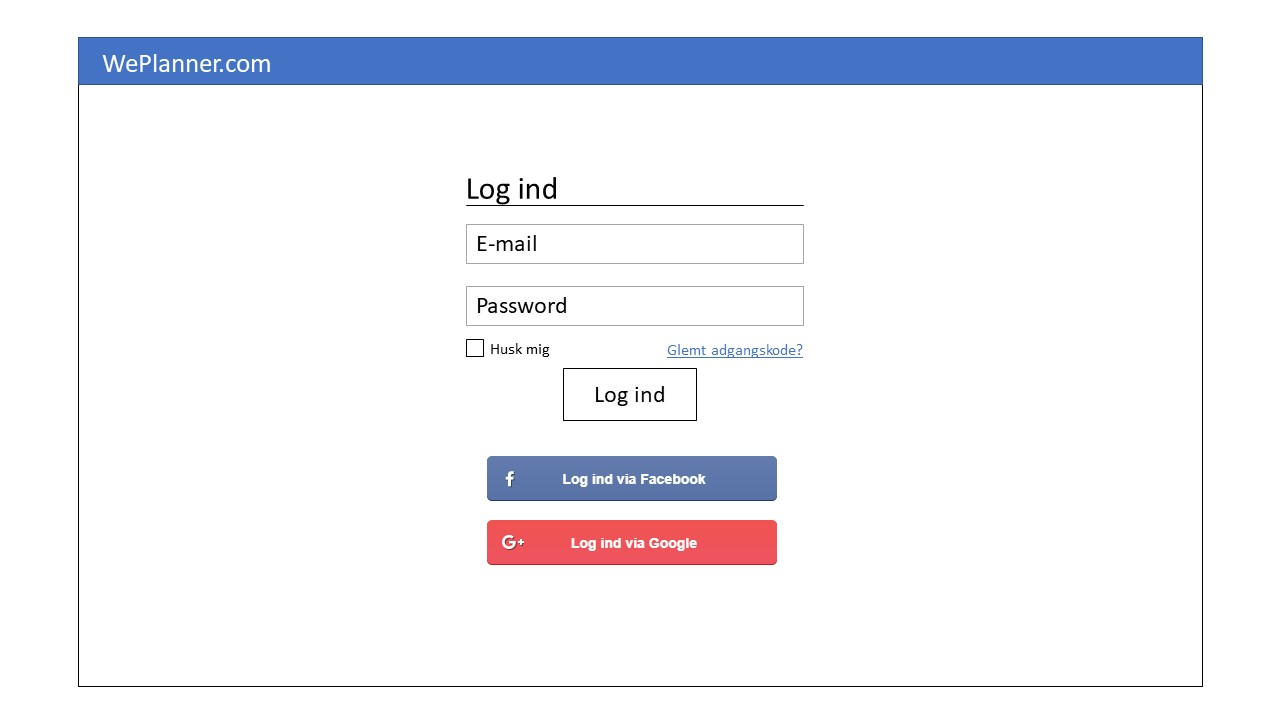
\includegraphics[width=\linewidth]{01_Indledning/Images/Slide1.JPG}
  \caption{Login side}
  \label{fig:login_site}
\end{figure}

\noindent Når man er logget ind med sin bruger, møder man 'Home' siden, som kan ses på figur \ref{fig:home_site}. Her kan brugeren se alle de grupper som brugeren er medlem af. Derudover har brugeren også mulighed for at oprette en gruppe.
\begin{figure}[H]
  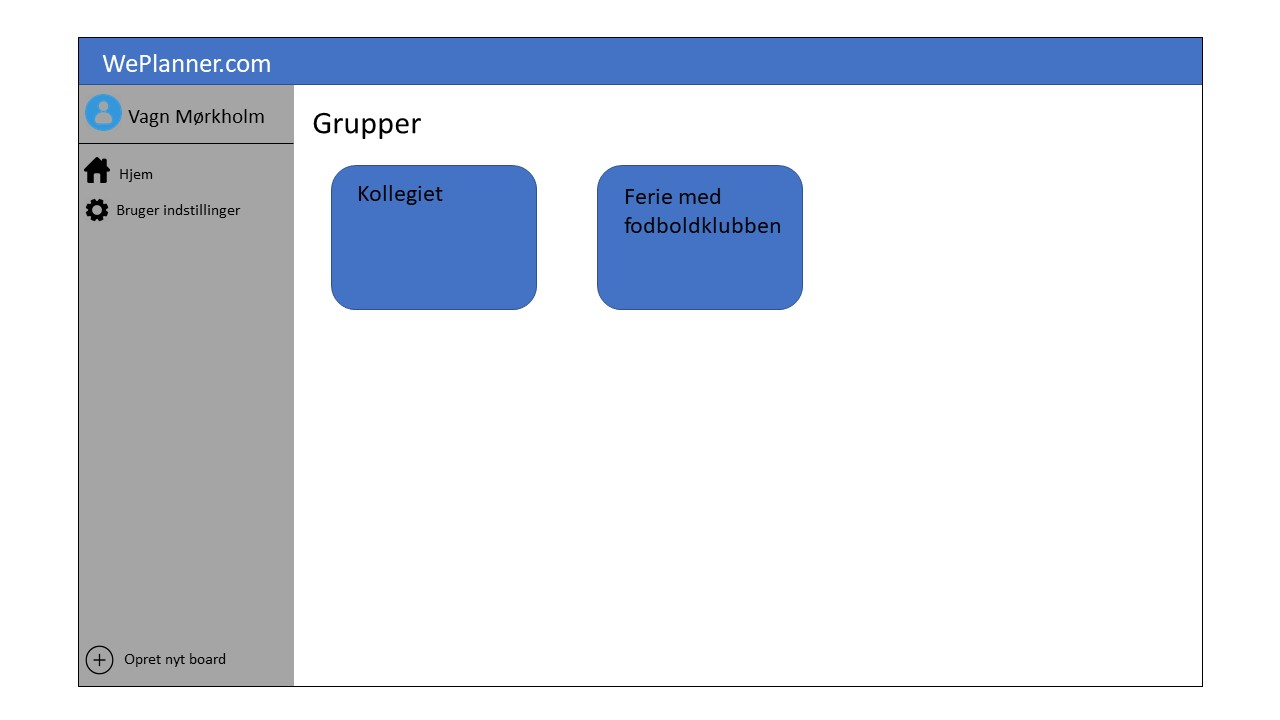
\includegraphics[width=\linewidth]{01_Indledning/Images/Slide2.JPG}
  \caption{Home side}
  \label{fig:home_site}
\end{figure}

\noindent Ved at vælge en gruppe, kommer man ind på en ny side som viser gruppen med alle de tilføjede widgets. Her kan brugeren få et hurtigt overblik ved at kigge på de forskellige widgets. Brugeren kan så trykke på en widget, som udvider sig og giver flere informationer. Dette ses på figur \ref{fig:board_site}.
\begin{figure}[H]
  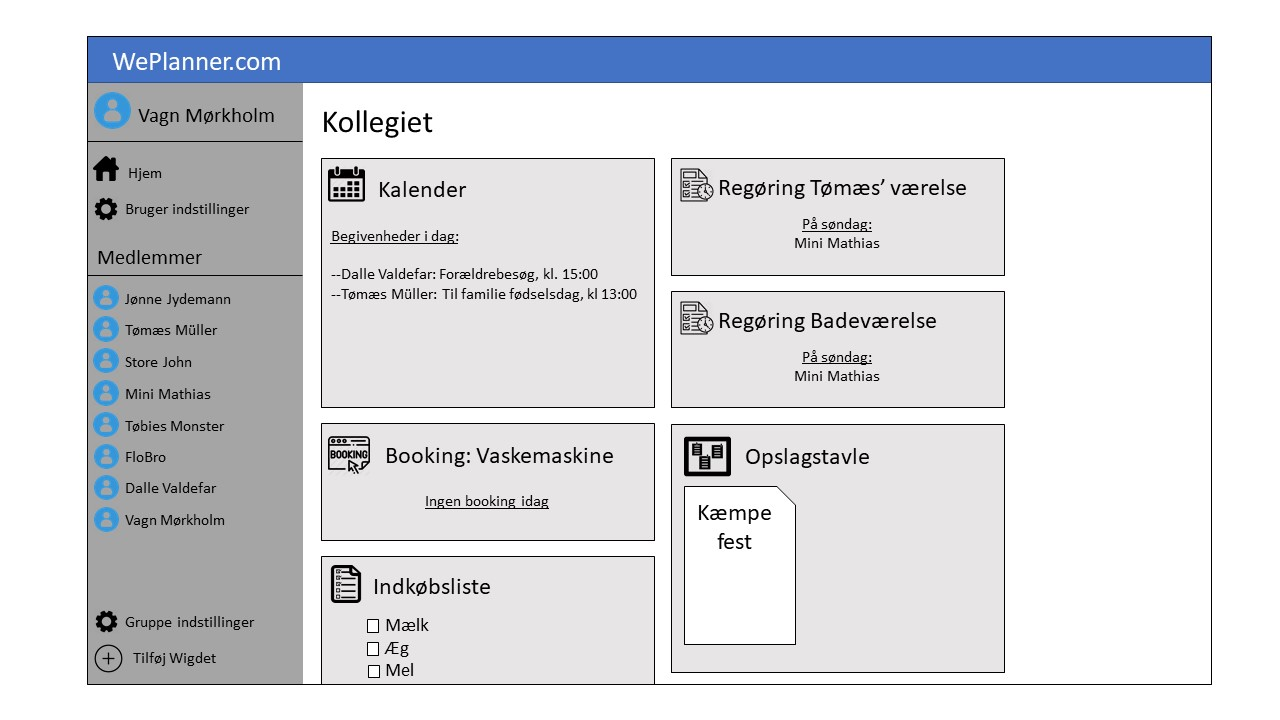
\includegraphics[width=\linewidth]{01_Indledning/Images/Slide3.JPG}
  \caption{Gruppe side}
  \label{fig:board_site}
\end{figure}